\documentclass[12pt, letterpaper, twoside]{article}
\usepackage[utf8]{inputenc}
\usepackage{amsmath}
\usepackage{amsfonts}
\usepackage{amssymb}
\usepackage{mathtools}
\usepackage[mathscr]{euscript}
\DeclarePairedDelimiter{\ceil}{\lceil}{\rceil}
\documentclass[pstricks,border=12pt]{standalone}
\usepackage{pst-plot}

\documentclass{article}
\usepackage{pgfplots}
\pgfplotsset{%
    ,compat=1.12
    ,every axis x label/.style={at={(current axis.right of origin)},anchor=north west}
    ,every axis y label/.style={at={(current axis.above origin)},anchor=north east}
    }


\begin{document}

Last Tuesday, we derived a representation for Euler's constant $\gamma$, where 

\begin{equation}
    \gamma = 1 - \int_{1}^\infty \frac{\{t\}}{t^2} dt
\end{equation}

We posed the question of how we would integrate such a function. I provide one idea here. \\

Let $\{x\}$ denote the fractional part of $x$, where $\{x\} = x - \lfloor x \rfloor$. Graphing this function yields a sawtooth-like shape. \\

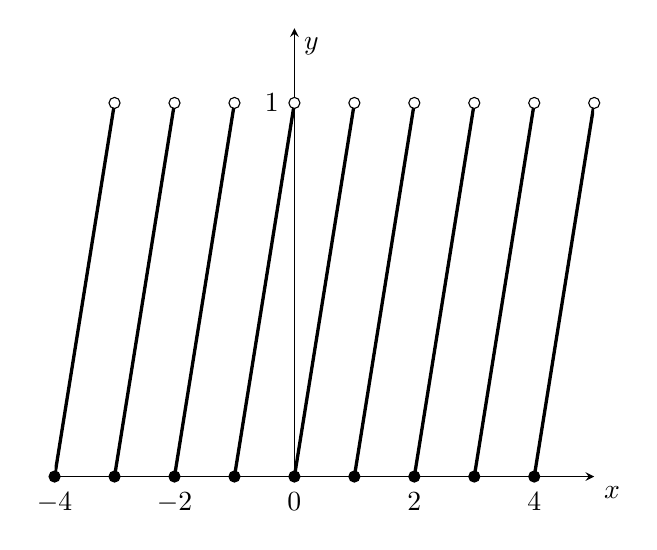
\begin{tikzpicture}

\tikzset{
  jumpdot/.style={mark=*,solid},
  excl/.append style={jumpdot,fill=white},
  incl/.append style={jumpdot,fill=black},
}

\begin{axis}[%
    ,xlabel=$x$
    ,ylabel=$y$
    ,axis x line = bottom,axis y line = middle
    ,ytick={0, 1, 2}
    ,ymax=1.2 % or enlarge y limits=upper
    ]
\addplot[incl] coordinates {(-4, 0)};    
\addplot [very thick, smooth,samples=200,color=black] table {
-4 0
-3 1
};
\addplot[incl] coordinates {(-3, 0)};
\addplot [very thick, smooth,samples=200 ,color=black] table {
-3 0
-2 1
};
\addplot[incl] coordinates {(-2, 0)};
\addplot [very thick, smooth,samples=200 ,color=black] table {
-2 0
-1 1
};
\addplot[incl] coordinates {(-1, 0)};
\addplot [very thick, smooth,samples=200 ,color=black] table {
-1 0
0 1
};
\addplot[incl] coordinates {(0, 0)};
\addplot [ very thick, smooth,samples=200,color=black] table {
0 0 
1 1
};
\addplot[incl] coordinates {(1, 0)};
\addplot [very thick, smooth,samples=200 ,color=black] table {
1 0 
2 1
};
\addplot[incl] coordinates {(2, 0)};
\addplot [very thick, smooth,samples=200 ,color=black] table {
2 0
3 1
};
\addplot[incl] coordinates {(3, 0)};
\addplot [ very thick, smooth,samples=200,color=black] table {
3 0
4 1
};
\addplot[incl] coordinates {(4, 0)};
\addplot [very thick, smooth,samples=200,color=black] table {
4 0
5 1
};
\addplot[excl] coordinates {(-3, 1)};
\addplot[excl] coordinates {(-2, 1)};
\addplot[excl] coordinates {(-1, 1)};
\addplot[excl] coordinates {(0, 1)};
\addplot[excl] coordinates {(1, 1)};
\addplot[excl] coordinates {(2, 1)};
\addplot[excl] coordinates {(3, 1)};
\addplot[excl] coordinates {(4, 1)};
\addplot[excl] coordinates {(5, 1)};
\end{axis}
\end{tikzpicture}

Note that the function is continuous on $\mathbb{R} / \mathbb{Z}$. With this in mind, we can break up the integral so that we need only integrate on the parts of the function that are continuous. Let us turn our view to one of many ``lines" on this function. For example, the ``line" stemming from the origin is simply the function $f(x) = x$ over the domain $[0, 1)$. In fact, the general equation for any line stemming from the point $(k, 0)$ is the function $f_k(x) = x - k$ defined over the domain $[k, k+1)$. Even though we have not covered the Riemann integral, we can take the following theorem as true. \\

From Abbott: 
If $f \colon [a, b] \rightarrow \mathbb{R}$ is bounded, and $f$ is integrable on $[c, b]$ for
all $c \in (a, b)$, then $f$ is integrable on $[a, b]$. An analogous result holds at the
other endpoint. \\

\newpage

Our equation for $\gamma$ becomes 

\begin{equation}
    \gamma = 1 - \sum_{n=1}^\infty \int_{n}^{n+1} \frac{f_n(t)}{t^2} dt
\end{equation}

Some algebraic manipulation yields 

\begin{equation}
\begin{split}
    \gamma &= 1 - \sum_{n=1}^\infty \int_{n}^{n+1} \frac{f_n(t)}{t^2} dt \\
    &= 1 - \sum_{n=1}^\infty \int_{n}^{n+1} \frac{t - n}{t^2} dt \\
    &= 1 - \sum_{n=1}^\infty \int_{n}^{n+1} \frac{t}{t^2}  - \frac{n}{t^2} dt \\
    &= 1 - \sum_{n=1}^\infty \int_{n}^{n+1} \frac{1}{t} - \frac{n}{t^2} dt \\
    &= 1 - \sum_{n=1}^\infty \ln t + \frac{n}{t} \Big|_n^{n+1} \\
    &= 1 - \sum_{n=1}^\infty \bigg(\ln (n+1) + \frac{n}{n+1}\bigg) - \bigg(\ln n + \frac{n}{n}\bigg) \\
\end{split}
\end{equation}

Some properties of logarithms yields 

\begin{equation}
    \gamma = 1 - \sum_{n=1}^\infty \bigg[\ln \bigg(1 + \frac{1}{n}\bigg) - \frac{1}{n+1}\bigg]
\end{equation}



\end{document}
